\documentclass{beamer}
\usepackage[utf8]{inputenc}
\usetheme{Madrid}
\usecolortheme{beaver}


\usepackage[english]{babel}
\usepackage{graphicx}
\usepackage{amssymb}
\usepackage{amsmath}
\usepackage{bbm}
\usepackage{svg}
\usepackage{tikz}
\usetikzlibrary{calc}
\usetikzlibrary{arrows}
\usepackage{amsfonts}
\usepackage{mathtools}
\usepackage{pgfplots}
\usepackage{xcolor}
\usepackage{comment}
\usepackage{float}
\usepackage{csvsimple}
\usepackage[authoryear,round]{natbib}
\usepackage{hyperref}
\usepackage{threeparttable}
\usepackage{booktabs}
\usepackage{multirow}
\usepackage{dcolumn}
\usepackage{longtable}


\usetikzlibrary{automata,arrows,positioning,calc}
\usetikzlibrary{plotmarks}
\usetikzlibrary{decorations.pathreplacing}

\newcolumntype{.}{D{.}{.}{-1}}

\setbeamertemplate{navigation symbols}{}

\pgfplotsset{compat=1.17}

\hypersetup{
    colorlinks=true,
    linkcolor=blue,
    filecolor=magenta,
    urlcolor=blue,
    citecolor=blue,
}

\graphicspath{{plots/}{../output/plots/}{images/}}
\makeatletter
\def\input@path{{tables/}{../output/tables/}}
\makeatother


\title[Market Run Psychology]{To Sell or not to Sell:\\ The Psychology of Market Runs}


\author[Eynon \& Jindapon]{Caleb Eynon and Paan Jindapon}

\institute[]{
  University of Alabama
}

\date[5/27/2026] % (optional)
{
Beijing Normal–Hong Kong Baptist University
\\
May 27th, 2026

}

\logo{
\includegraphics[height=1.0cm]{A-Square.eps}}

\begin{document}

\frame{\titlepage}

%%%%%%%%%%%%%%%%%%%%%%%%%%%%%%%%%%%%%
\section{Introduction}
%%%%%%%%%%%%%%%%%%%%%%%%%%%%%%%%%%%%%

\begin{frame}{Motivation}

 Financial volatility and panic-induced liquidation are recurring features of crises
        \begin{itemize}
        \item U.S. Liberation Day (April, 2 2025):  Dow fell 9\% the next day
        \item COVID-19 lockdowns (March 2020): Dow fell 26\% in four days
        \item Black Monday (October 19, 1987): Dow fell 22.6\% in one day
        \end{itemize}

\end{frame}

\begin{frame}{Motivation}


\begin{center}
``Panics,'' ``frenzies,'' and ``manias'' in financial markets \\ are \textbf{emotional} responses.  

\vspace{0.4in}


\includegraphics[width=6cm]{images/MF-INSIDE-OUT-2-COMP.png}


Which emotions?

\end{center}

\end{frame}


\begin{frame}{Research Questions}
\begin{itemize}
    \item Market runs: Panic investors sell too soon
            \begin{itemize}
        \item How much do investors \textbf{overreact} to bad news?
        \item Do investors herd?
        \end{itemize}
    \item What psychological factors predict participation in market runs?
        \begin{itemize}
        \item Personal traits
        \item Primary emotions
        \end{itemize}
    \item Can communication mitigate market runs?
    
\end{itemize}
\end{frame}


\begin{frame}{Background}

\textbf{Bank Runs}

\vspace{0.1in}

\begin{itemize}
    \item \cite{diamond1983bank}
    \item \textbf{Some} players suffer individual liquidity shocks
    \item Bank-run equilibrium: \textbf{All} players withdraw early
\end{itemize}

\vspace{0.2in}

\textbf{Market Runs}

\vspace{0.1in}

\begin{itemize}
    \item \cite{bernardo2004liquidity}
    \item Possibility of liquidity shocks in the future
%    \item Each sale \textbf{immediately} lowers price
    \item Market-run equilibrium: \textbf{All}  players sell early
\end{itemize}

\end{frame}


\begin{frame}{Bank Runs in the Lab}
\begin{itemize}
    \item \cite{schotter2009dynamics}:     
    \begin{itemize}
        \item Dynamic bank-run game, group of 6, 4 periods, 21 rounds, simultaneous VS sequential, symmetric VS asymmetric info.
        \item Herding is observed.
        \end{itemize}
    \vspace{0.2in}
    \item \cite{dijk2017bank}: 
    \begin{itemize}
        \item Induces fear, happy, sadness prior to static bank-run game. 
        \item Fear inducement increases withdrawal probability
    \end{itemize}
    %\item \cite{shakina2018coordination}: Communication slows withdrawals
\end{itemize}
\end{frame}


\begin{frame}{Market Runs in the Lab}
\begin{itemize}
    \item \cite{magnani2020dynamic}: 
    \begin{itemize}
        \item First experimental implementation of \cite{bernardo2004liquidity}. \item 80 subjects, group of 4, 55 rounds. $2\times2$ treatments: with and without circuit breakers and high or low public signal quality.
        \item Findings: Circuit-breakers improve welfare given high signal quality
    \end{itemize}
        \vspace{0.1in}
    \item \cite{choi2022market}: 
        \begin{itemize}
        \item 84 subjects, group of 4, 50 rounds. 3 treatments: low/medium/high market liquidity.
        \item Findings: Less liquid, more runs.
        \end{itemize}
        \vspace{0.1in}
    \item \cite{kendall2020market}: 
            \begin{itemize}
        \item Different framework 
        \item 64 subjects. group of 8, 8 periods, 30 rounds. 2 treatments: low and high quality of private signals. Subjects must either buy or (short) sell.
        \item  Findings: excessive early trading
        \end{itemize}
\end{itemize}
\end{frame}


\begin{frame}{ Personality Traits}

\textbf{The Big Five}

    \begin{itemize}
    \item \textbf{O}penness: willingness to embrace new ideas or  experiences
    \item \textbf{C}onscientiousness: being responsible, organized, and reliable
    \item \textbf{E}xtraversion: being outgoing, energetic, and social
    \item \textbf{A}greeableness: tendency to avoid conflict and cooperate
    \item \textbf{N}euroticism: emotional instability, anxiety
    \end{itemize}
\end{frame}


\begin{frame}{Traits and Emotions}
 
\begin{itemize}
    \item Neuroticism $\rightarrow$ lower risk tolerance \citep{rustichini2016toward}
    \item Conscientiousness $\rightarrow$ higher trading volume \citep{bajo2023psychological}
    \item Conscientiousness $\rightarrow$ less cooperation \citep{proto2019intelligence}
    \item Anxiety $\rightarrow$ conservative financial decisions \citep{gambetti2012effect}
\end{itemize}
\end{frame}

\begin{frame}{Facial expressions}
 
\begin{itemize}
    \item Positive emotional state correlates with purchases and overpricing. Fear correlates with selling, low prices, and price decreases \citep{breaban2018emotional}
    
    \item   Positive emotions (joy and valence) and risk tolerance are positively correlated \citep{kassas2022happy}

    \item In a public-good game, having contributed more than others and anger are positively  correlated \citep{noussair2024role}
\end{itemize}
\end{frame}


\begin{frame}{What We Do}
\begin{itemize}
    \item Experimentally implement \cite{bernardo2004liquidity} theoretical framework with \cite{magnani2020dynamic} experimental design
    \item Measure \textbf{personality traits} via validated surveys (TIPI, BIS-11, STAI)
    \item Measure \textbf{primary emotions} via facial reading technology (Affectiva)
    \item 2$\times$2 mixed design:
    \begin{itemize}
        \item \textbf{Within-subjects}: without and with communication
        \item \textbf{Between-subjects}:  multiple random prices vs single average price in batch trading (tie-breaking rules for selling in the same period)
    \end{itemize}
    %\item 6 sessions, 96 subjects, 720 group-rounds
\end{itemize}
\end{frame}



\begin{frame}{Preview of Results}
\begin{enumerate}

    \item \textbf{Personality traits}
\begin{itemize}
    \item Positive effects: conscientiousness, anxiety 
    \item Negative effects: agreeableness, risk tolerance
\end{itemize}   

    \item \textbf{Primary Emotions}
\begin{itemize}
    \item Positive effects: disgust
    \item Negative effects: joy, valence
\end{itemize}   


    \item \textbf{Communication reduces runs:}  fewer sellers and later first sales when subjects are allowed to chat.

    \item \textbf{Market clearing price matters:} more runs under average price rule. 
        
    \item \textbf{Emotional Herding:} Yes!
    \begin{itemize}
    \item Positive effects: fear
    \item Negative effects: surprise
\end{itemize}   
 %   \item \textbf{Luck matters:} ``Lucky'' liquidation payoffs decrease future selling
\end{enumerate}
\end{frame}


%%%%%%%%%%%%%%%%%%%%%%%%%%%%%%%%%%%%%
\section{The Model}
%%%%%%%%%%%%%%%%%%%%%%%%%%%%%%%%%%%%%

\begin{frame}{Market Model}
\begin{itemize}
    \item $4$ investors in a market round, each endowed with one asset with the value of 20 units.
    \item Each market round has multiple market periods.  
    \begin{itemize}
    \item Each investor can sell the asset at market price in any period.
    \item Number of market periods is random. 
    \item Termination probability after each period is  $0.125$.
    \end{itemize} 
    
    \item Two possible states of the world for each market round
     \begin{itemize}
    \item Good ($G$) and Bad ($B$) with an equal chance ($50/50$)
    \end{itemize} 
    

\end{itemize}
\end{frame}


\begin{frame}{Market Model}
\begin{itemize}
    \item The state of the world will be revealed at the end of the round. 
     \begin{itemize}
     \item Each will receive the asset value (20 units) in Good state. 
     \item Each will be forced to sell the asset at market price in Bad state.
     \end{itemize}
     
 \item Market price schedule: $p_n = 2n$
    \begin{center}
    \begin{tabular}{cc} 
    \toprule
    \textbf{Investors remaining ($n$)} & \textbf{Price  ($p_n$)} \\
    \midrule
    4 & 8 \\
    3 & 6 \\
    2 & 4 \\
    1 & 2 \\
    \bottomrule
    \end{tabular}
    \end{center}

\end{itemize}
\end{frame}


\begin{frame}{Market Model}
\begin{itemize}

    \item At the beginning of each period, all investors receives a noisy binary signal ($g$ or $b$) about the state.
    \item Signal accuracy: \\$Prob( signal = g|state = G ) =  Prob( signal = b|state = B ) = 0.675$
    \item In each period, each investors update their belief about the state of the world and decide whether \textbf{to sell or not to sell} the asset.
\end{itemize}
\end{frame}


\begin{frame}{Bayesian Updating}
\begin{itemize}
    \item $\pi(t)$ is the posterior belief of $Prob(state = G)$ in period $t$  
    \item $y(t)$ is public signal in period $t$  
\end{itemize}

\begin{equation*}
    \pi(t) :=
    \begin{cases}
        \dfrac{\pi(t\!-\!1) \times 0.675}{\pi(t\!-\!1)\times 0.675 + (1\!-\!\pi(t\!-\!1))\times 0.325}, & \text{if } y(t) = g \\[12pt]
        \dfrac{\pi(t\!-\!1)\times 0.325}{\pi(t\!-\!1)\times 0.325 + (1\!-\!\pi(t\!-\!1))\times 0.675}, & \text{if } y(t) = b
    \end{cases}
\end{equation*}

\vspace{0.1in}

\begin{itemize}
    \item $\pi(0) = 0.5$ (common prior)
    \item $\pi(t) \overset{a.s.}{\to} 1$ if Good state; $\pi(t) \overset{a.s.}{\to} 0$ if Bad state
\end{itemize}
\end{frame}


\begin{frame}{Equilibrium}

\begin{itemize}
    \item If all assets are owned by a risk-neutral mutual fund manager, they should never sell. 
    \item Symmetric equilibrium strategy is mixed.
    \item If all investors are risk neutral, the first sale will occur when the posterior belief is lower than $1/3$ and higher than $1/5$.
    
\end{itemize}
\end{frame}


%%%%%%%%%%%%%%%%%%%%%%%%%%%%%%%%%%%%%
\section{The Experiment}
%%%%%%%%%%%%%%%%%%%%%%%%%%%%%%%%%%%%%

\begin{frame}{ }
 \begin{center}
     \textbf{The Experiment}
 \end{center}
\end{frame}


\begin{frame}{Implementation}
\begin{itemize}
    \item TIDE Lab, University of Alabama
    \item SONA recruitment, October-December, 2025
    \item IRB approved and preregistered
    \item  6 sessions $\times$ 16 subjects = 96 total subjects
    \item Show-up fee: 7.50 USD for 75-minute session
    \item Part 1: Market runs (8-80 Experimental Currency Units) 
    \item Part 2: Personality survey (0-50 Experimental Currency Units) 
    \item Conversion rate: 4 ECU = 1 USD
    \item Possible total earnings: 9.50-40.00 USD (actual average 23.57 USD)
\end{itemize}
\end{frame}


\begin{frame}{Part 1: Market Runs}
\begin{itemize}
    \item Each session: 4 segments   
    \item Each segment: uncertain number of market rounds
    \item Each round: uncertain number of market periods  
    \item Each period: 4 seconds   
    \item Group assignment: groups of 4, reshuffled each segment, no repeated interaction with another participant across segments
\end{itemize}

\vspace{0.3cm}
\begin{center}
\begin{tabular}{ccc}
\toprule
& \textbf{Segments 1--2} & \textbf{Segments 3--4} \\
\midrule
\textbf{Treatment 1} (Random Price) & No chat & Chat \\
\textbf{Treatment 2} (Average Price) & No chat & Chat \\
\bottomrule
\end{tabular}
\end{center}
\end{frame}


\begin{frame}{Treatments (Between Subjects)}

\textbf{Random Price VS Average Price}

imposed when 
\begin{itemize}
    \item multiple sellers in a market period, or 
    \item multiple investors liquidate at the end of round (in Bad state).
\end{itemize}

\vspace{0.2in}

\textbf{Example 1:} Suppose at time $t-1$, no one has sold. In period $t$, Players A and B both sell.

\vspace{0.1in}

\textbf{Treatment 1 (Random Price):}
\begin{itemize}
    \item Either A gets $8$ and B gets $6$, or A gets $6$ and B gets  $8$ (50/50)
\end{itemize}

\vspace{0.1in}

\textbf{Treatment 2 (Average Price):}
\begin{itemize}
    \item Both get $\bar{p} = (8+6)/2 = 7$
\end{itemize}

\end{frame}

\begin{frame}{Treatments (Between Subjects)}

\textbf{Random Price VS Average Price}

imposed when 
\begin{itemize}
    \item multiple sellers in a market period, or 
    \item multiple investors liquidate at the end of round (in Bad state).
\end{itemize}

\vspace{0.2in}

\textbf{Example 2:} Suppose market round has ended and the state for the round is Bad.  A have B have sold. C and D hold the asset at the end.

\vspace{0.1in}

\textbf{Treatment 1 (Random Price):}
\begin{itemize}
    \item Either C gets $4$ and D gets $2$, or C gets $2$ and D gets $4$ (50/50)
\end{itemize}

\vspace{0.1in}

\textbf{Treatment 2 (Average Price):}
\begin{itemize}
    \item Both get $\bar{p} = (4+2)/2 = 3$
\end{itemize}

\end{frame}

\begin{frame}{Treatments (Between Subjects)}

\textbf{Random Price VS Average Price}

\begin{itemize}
    \item Random price is a mean-preserving spread of Average price.
    \item Risk-neutral investors are indifferent.
    \item In Bad state, holding under Average Price (5) has a higher expected utility than under Random price (8/6/4/2) for a risk-averse investor
    \item But which one induces more incentive to deviate from holding?
    \item So the expected utility gained from deviating is larger under Average Price (3) than  under Random Price (0/2/4/6) for a risk-averse investor
\end{itemize}




\end{frame}

\begin{frame}{Treatments (Within Subjects)}

\textbf{Communication}

\begin{itemize}
    \item  Subjects can chat within their group for 90 seconds at the beginning of Segment 3 and Segment 4.
    \item They did not know that they were allowed to chat until after Segment~2.
    \item Within-subjects design to avoid idle time under ``No Communication'' treatment which may affect emotions.
\end{itemize}

\end{frame}


\begin{frame}{Important Features}

\begin{itemize}
    \item 4 payment rounds: the computer randomly selects only 1 round \\from each segment to calculate cash payment.
    \item Utilized video instructions: \href{https://youtu.be/5h83uTS_RMc}{link} (show 0:29 to 1:24) 
    \item After the instructions, subjects complete a quiz, average of 85\% correct first attempt
    \item Facial motion recording via webcams throughout the experiment
\end{itemize}
\end{frame}


\begin{frame}{Part 1 Summary}
\begin{center}
\begin{minipage}{10cm}
% Experiment flow diagram: hierarchical tree showing session structure
% Session -> Segments -> Rounds -> Periods
% Uses TikZ libraries: automata, arrows, positioning, calc (loaded in main.tex)

\begin{figure}[H]
\centering
\resizebox{\textwidth}{!}{%
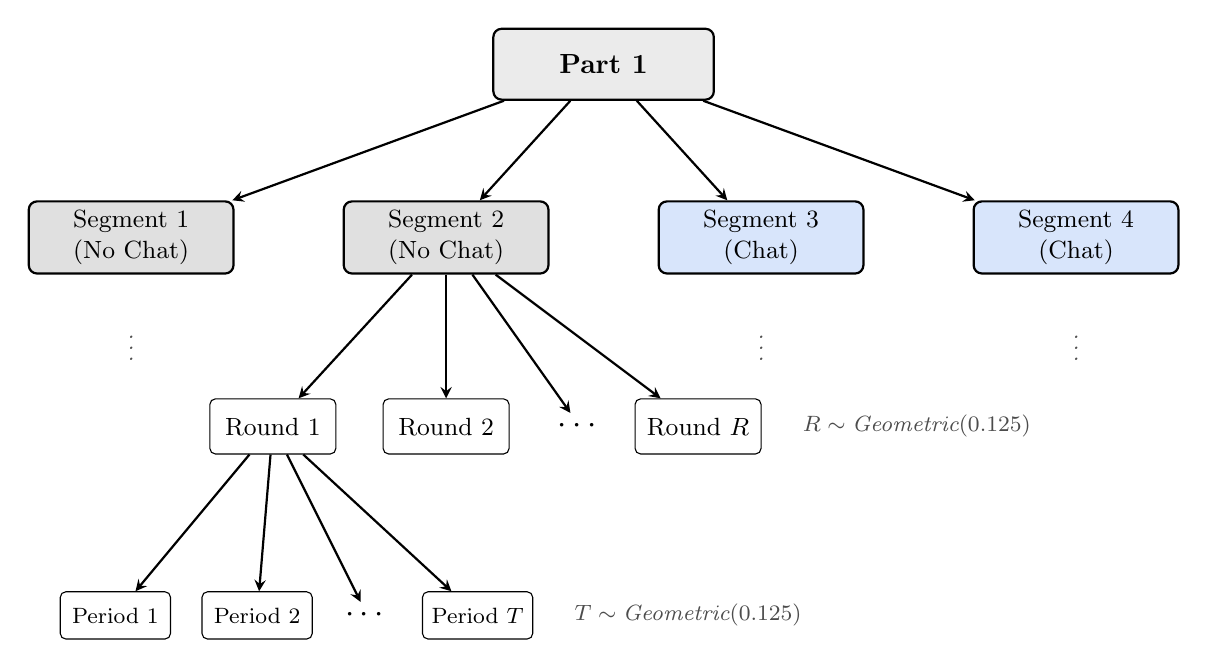
\begin{tikzpicture}[
    % Node styles
    session/.style={
        rectangle, draw, thick, rounded corners=3pt,
        fill=black!8, minimum width=2.8cm, minimum height=0.9cm,
        font=\bfseries\normalsize
    },
    nochat/.style={
        rectangle, draw, thick, rounded corners=3pt,
        fill=black!12, minimum width=2.6cm, minimum height=0.8cm,
        font=\small, align=center
    },
    chat/.style={
        rectangle, draw, thick, rounded corners=3pt,
        fill=CornflowerBlue!25, minimum width=2.6cm, minimum height=0.8cm,
        font=\small, align=center
    },
    roundnode/.style={
        rectangle, draw, rounded corners=2pt,
        fill=white, minimum width=1.6cm, minimum height=0.7cm,
        font=\small
    },
    periodnode/.style={
        rectangle, draw, rounded corners=2pt,
        fill=white, minimum width=1.4cm, minimum height=0.6cm,
        font=\footnotesize
    },
    ellipsisnode/.style={
        font=\large, inner sep=2pt
    },
    annotation/.style={
        font=\footnotesize\itshape, text=black!70
    },
    arrowed/.style={
        ->, >=stealth, thick
    },
]

% === Session node ===
\node[session] (session) {Part 1};

% === Segment nodes (evenly spaced using absolute x-coordinates) ===
\node[nochat] (seg1) at (-6, -2.2) {Segment 1\\(No Chat)};
\node[nochat] (seg2) at (-2, -2.2) {Segment 2\\(No Chat)};
\node[chat]   (seg3) at ( 2, -2.2) {Segment 3\\(Chat)};
\node[chat]   (seg4) at ( 6, -2.2) {Segment 4\\(Chat)};

% === Session -> Segment edges ===
\draw[arrowed] (session) -- (seg1);
\draw[arrowed] (session) -- (seg2);
\draw[arrowed] (session) -- (seg3);
\draw[arrowed] (session) -- (seg4);

% === Vertical dots under segments without expanded subtree ===
\node[annotation] at (-6, -3.5) {$\vdots$};
\node[annotation] at ( 2, -3.5) {$\vdots$};
\node[annotation] at ( 6, -3.5) {$\vdots$};

% === Round nodes (under Segment 2) ===
\node[roundnode] (r1) at (-4.2, -4.6) {Round 1};
\node[roundnode] (r2) at (-2.0, -4.6) {Round 2};
\node[ellipsisnode] (rdots) at (-0.3, -4.6) {$\cdots$};
\node[roundnode] (rR) at (1.2, -4.6) {Round $R$};

% === Segment -> Round edges ===
\draw[arrowed] (seg2) -- (r1);
\draw[arrowed] (seg2) -- (r2);
\draw[arrowed] (seg2) -- (rdots);
\draw[arrowed] (seg2) -- (rR);

% === Geometric annotation for rounds ===
\node[annotation, right=0.4cm of rR]
    {$R \sim \text{Geometric}(0.125)$};

% === Period nodes (under Round 1) ===
\node[periodnode] (p1) at (-6.2, -7.0) {Period 1};
\node[periodnode] (p2) at (-4.4, -7.0) {Period 2};
\node[ellipsisnode] (pdots) at (-3.0, -7.0) {$\cdots$};
\node[periodnode] (pT) at (-1.6, -7.0) {Period $T$};

% === Round -> Period edges ===
\draw[arrowed] (r1) -- (p1);
\draw[arrowed] (r1) -- (p2);
\draw[arrowed] (r1) -- (pdots);
\draw[arrowed] (r1) -- (pT);

% === Geometric annotation for periods ===
\node[annotation, right=0.4cm of pT]
    {$T \sim \text{Geometric}(0.125)$};

\end{tikzpicture}%
}% end resizebox
\caption{Hierarchical structure of the experiment.}
\label{fig:experiment_flow}
\end{figure}

\end{minipage}
\end{center}
\end{frame}


\begin{frame}{Predetermined randomization}

\begin{table}[]\footnotesize
    \centering
\begin{tabular}{ccccc}
\toprule
Segment &Rounds & Periods per Round & Total Periods & Avg per Rnd \\
\midrule
  1  & 10 & 3, 10, 8, 4, 2, 3, 9, 7, 4, 6 & 56 & 5.6 \\
  2 & 5 & 9, 2, 5, 6, 5 & 27 & 5.4 \\
  3 & 6 & 9, 8, 4, 4, 3, 5 & 33 & 5.5 \\
  4 & 9 & 5, 3, 11, 3, 6, 14, 6, 3, 1 & 52 & 5.8 \\
\midrule
 \multicolumn{1}{c}{Total}  & 30 & --- & 168 & --- \\
 \multicolumn{1}{c}{ Avg per Seg} & 7.5 & --- & 42.0 & 5.6 \\
\bottomrule
\end{tabular}

\end{table}
\end{frame}


\begin{frame}{Participant Interface}
\begin{center}
    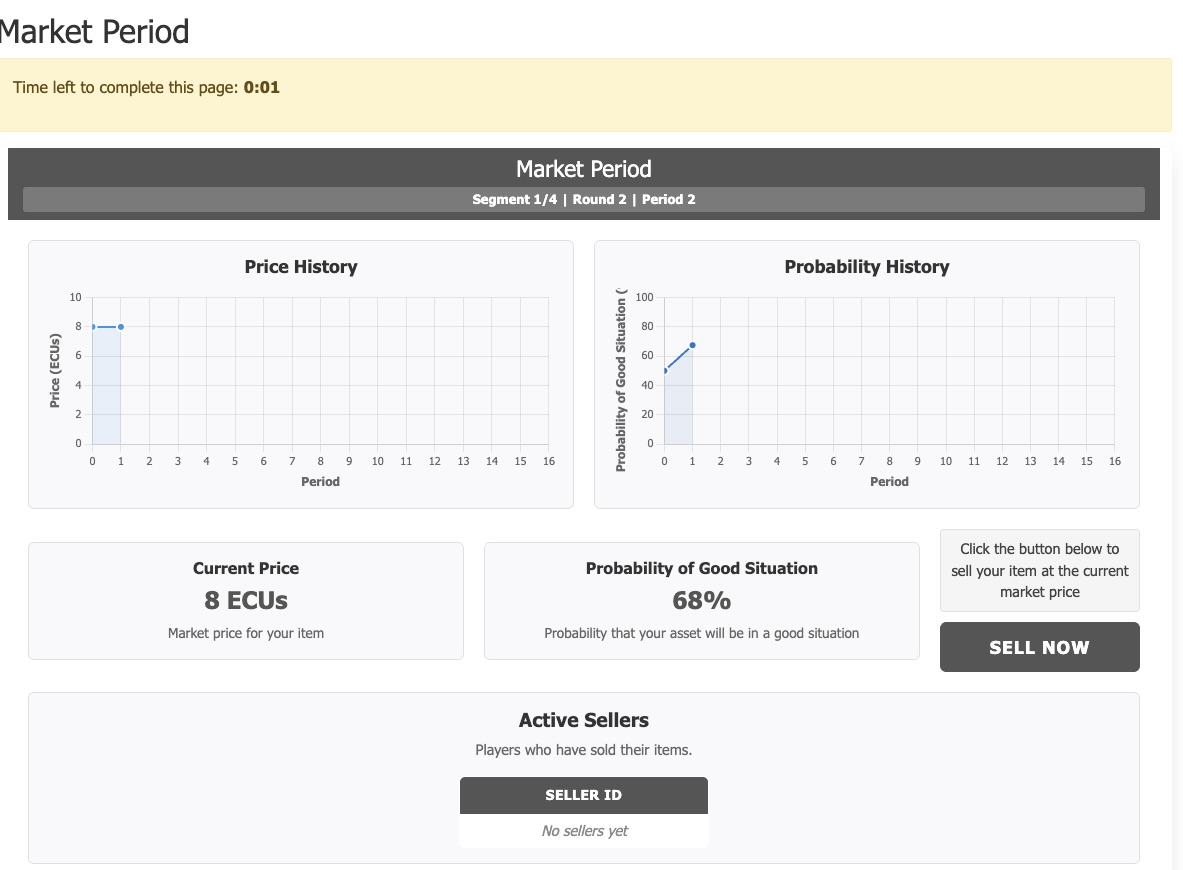
\includegraphics[width=0.85\linewidth]{interface.jpeg}
\end{center}
\end{frame}


\begin{frame}{Part 2: Survey}

\textbf{Five Sections}

\begin{enumerate}
    \item 6 questions (State-Trait Anxiety Inventory: I feel ...)
    \item 10 questions (Ten Item Personality Inventory: I see myself as ...)
    \begin{itemize}
    \item \textbf{O}penness 
    \item \textbf{C}onscientiousness 
    \item \textbf{E}xtraversion 
    \item \textbf{A}greeableness 
    \item \textbf{N}euroticism 
    \end{itemize}
    \item 8 questions (Barratt Impulsiveness Scale: I do ....  )
    \item 4 questions (age, gender, classification, major)
    \item 1 risk-taking task 
\end{enumerate}
   
\end{frame}

\begin{frame}{Part 2: Survey}

\textbf{Risk-taking Task} \citep{gneezy1997experiment}


\begin{itemize}
    \item  You will be asked to choose a portion of 20 ECUs that you earned from completing Sections 1 to 4 to invest in a risky option.  The rest of the earnings (those you do not invest) will be kept in your balance.

\vspace{0.1in}

    \item   There is a 50\% probability that the investment will fail and a 50\% probability that the investment will succeed. If the investment fails, you will lose the amount you invested. If the investment succeeds, you will receive 2.5 times the amount invested. 

\vspace{0.1in}

    \item   You will be asked to choose Heads or Tails. At the end of the study, we will flip a coin. Your investment succeeds if the outcome of the coin flip matches your choice. 

\end{itemize}
   
\end{frame}



\begin{frame}{Facial Expressions}


\textbf{Affectiva Software}


\begin{minipage}[0.5\textheight]{\textwidth}
\begin{columns}[T]
\begin{column}{0.05\textwidth}
\end{column}
\begin{column}{0.25\textwidth}
\vspace{0.2in}
\begin{itemize}
    \item Fear
    \item Anger
    \item Contemp
    \item Disgust
    \item Joy
    \item Sadness 
    \item Surprise
    \item Engagement
    \item Valence

\end{itemize}
\end{column}
\begin{column}{0.05\textwidth}
\end{column}
\begin{column}{0.7\textwidth}
\vspace{0.2in}
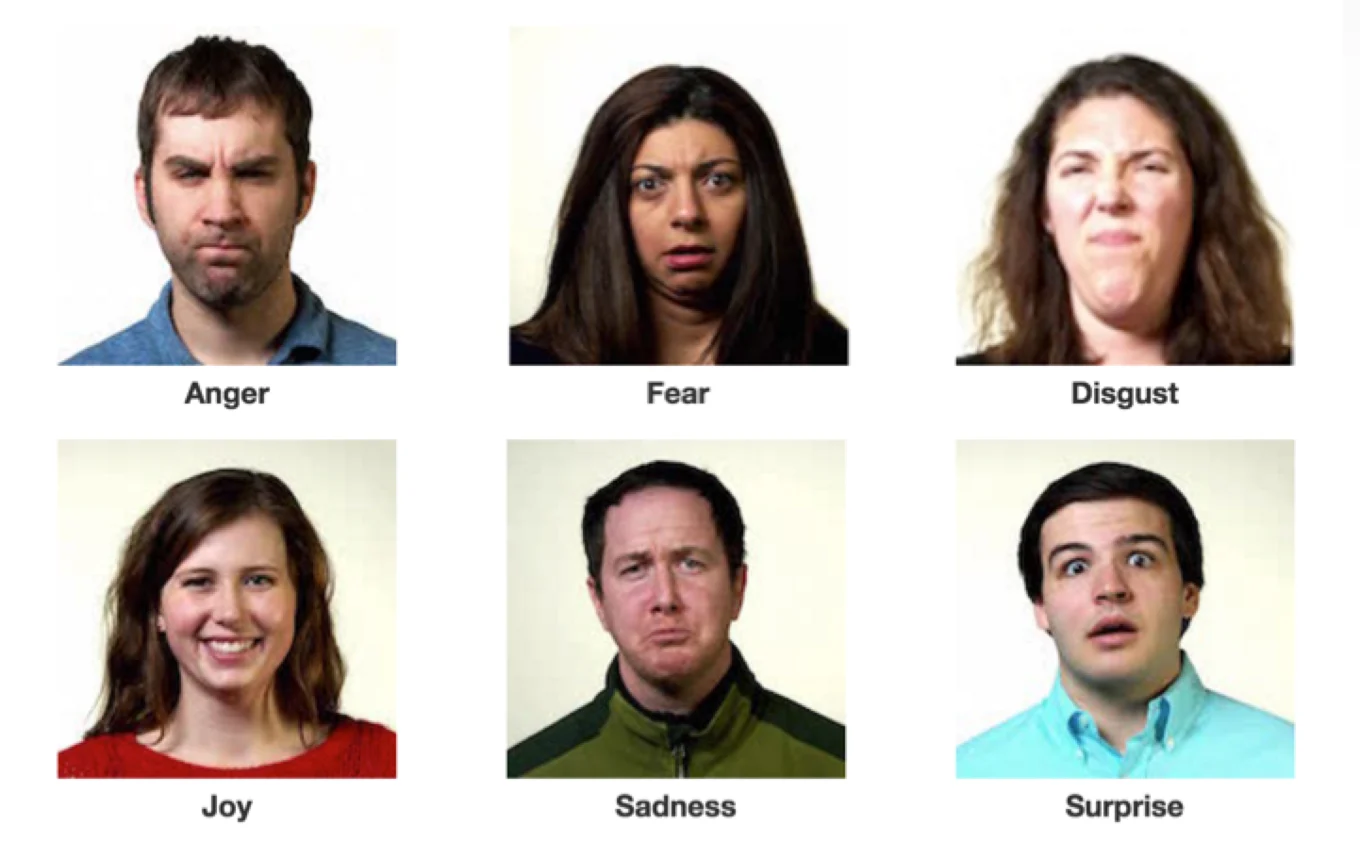
\includegraphics[width=8cm]{images/6_core_expressions.png}
\end{column}
\end{columns}
\end{minipage}

\end{frame}

%\begin{frame}{Facial Expressions}
%\begin{center}
%
\includegraphics[width=8cm]{images/aziz.png}


%Fear or Surprise?

%\end{center}
%\end{frame}


%%%%%%%%%%%%%%%%%%%%%%%%%%%%%%%%%%%%%
% HYPOTHESES
%%%%%%%%%%%%%%%%%%%%%%%%%%%%%%%%%%%%%

\begin{frame}{Hypotheses}
\textbf{H1:} Subjects are less likely to sell and less likely to sell early in the chat treatment than in the no-chat treatment.

\vspace{0.3cm}


\textbf{H2:} Subjects are more likely to sell early in the average-price treatment than in the random-price treatment.

\vspace{0.3cm}

\textbf{H3 (Personality Survey):}
\begin{itemize}
    \item \textcolor{red}{More likely to sell:} Impulsivity, anxiety, conscientiousness
    \item \textcolor{green!50!black}{Less likely to sell:} Agreeableness, risk tolerance, openness
\end{itemize}
\vspace{0.3cm}

\textbf{H4 (Facial Expressions):}
\begin{itemize}
    \item \textcolor{red}{More likely to sell:} Fear, anger, disgust, engagement
    \item \textcolor{green!50!black}{Less likely to sell:} Joy, valence
\end{itemize}
\end{frame}



%%%%%%%%%%%%%%%%%%%%%%%%%%%%%%%%%%%%%
\section{Results}
%%%%%%%%%%%%%%%%%%%%%%%%%%%%%%%%%%%%%

\begin{frame}{ }
 \begin{center}
     \textbf{Results}
 \end{center}
\end{frame}

\begin{frame}{Subject Pool}
\begin{center}
\scalebox{0.75}{
\begin{tabular}{lcccc}
\toprule
 & Range & Full Sample & Treatment 1 & Treatment 2 \\
  &   &   & Random Price & Average Price \\
\midrule
  $N$ (subjects) & & 96 & 48 & 48 \\
  $N$ (sessions) & & 6 & 3 & 3 \\
  Age & & 21.13 (3.23) & 21.21 (3.19) & 21.04 (3.30) \\
  Female (\%) & & 56.8 & 58.3 & 55.3 \\
\midrule
  Extraversion & [1,7] & 4.48 (1.48) & 4.31 (1.66) & 4.66 (1.26) \\
  Agreeableness & [1,7] & 4.83 (1.07) & 4.90 (1.09) & 4.77 (1.05) \\
  Conscientiousness & [1,7] & 5.57 (1.14) & 5.29 (1.13) & 5.85 (1.09) \\
  Neuroticism & [1,7] & 3.32 (1.43) & 3.49 (1.46) & 3.15 (1.38) \\
  Openness & [1,7] & 5.17 (1.12) & 5.21 (1.12) & 5.13 (1.12) \\
  Impulsivity & [1,7] & 3.09 (0.82) & 3.08 (0.79) & 3.10 (0.86) \\
  State Anxiety & [1,4] & 1.69 (0.55) & 1.65 (0.56) & 1.73 (0.55) \\
  Risk Tolerance & [0,20] & 11.80 (6.75) & 12.27 (6.44) & 11.32 (7.08) \\
\bottomrule
\end{tabular}
}

{\tiny\textit{Note:} Trait values as Mean (SD). Based on 95 survey respondents.}
\end{center}
\end{frame}




\begin{frame}{Selling Behavior}
\begin{center}
\scalebox{0.75}{
\begin{tabular}{lcccc}
\toprule
 & \multicolumn{2}{c}{Treatment 1} & \multicolumn{2}{c}{Treatment 2} \\
  & \multicolumn{2}{c}{Random Price} & \multicolumn{2}{c}{Average Price} \\
\cmidrule(lr){2-3} \cmidrule(lr){4-5}
 & Base & Chat & Base & Chat \\
\midrule
  Average number of sellers per group & 1.08 & 0.52 & 1.25 & 0.90 \\
  \quad Good state & 0.89 & 0.28 & 0.99 & 0.52 \\
  \quad Bad state & 1.40 & 0.70 & 1.52 & 1.23 \\
\midrule
  Average period of sales & 2.7 & 3.9 & 3.0 & 3.0 \\
  \quad Good state & 2.5 & 3.0 & 2.7 & 2.2 \\
  \quad Bad state & 3.0 & 4.2 & 3.2 & 3.3 \\
\bottomrule
\end{tabular}
}
\end{center}
\end{frame}



\begin{frame}{Selling Behavior}
\begin{center}
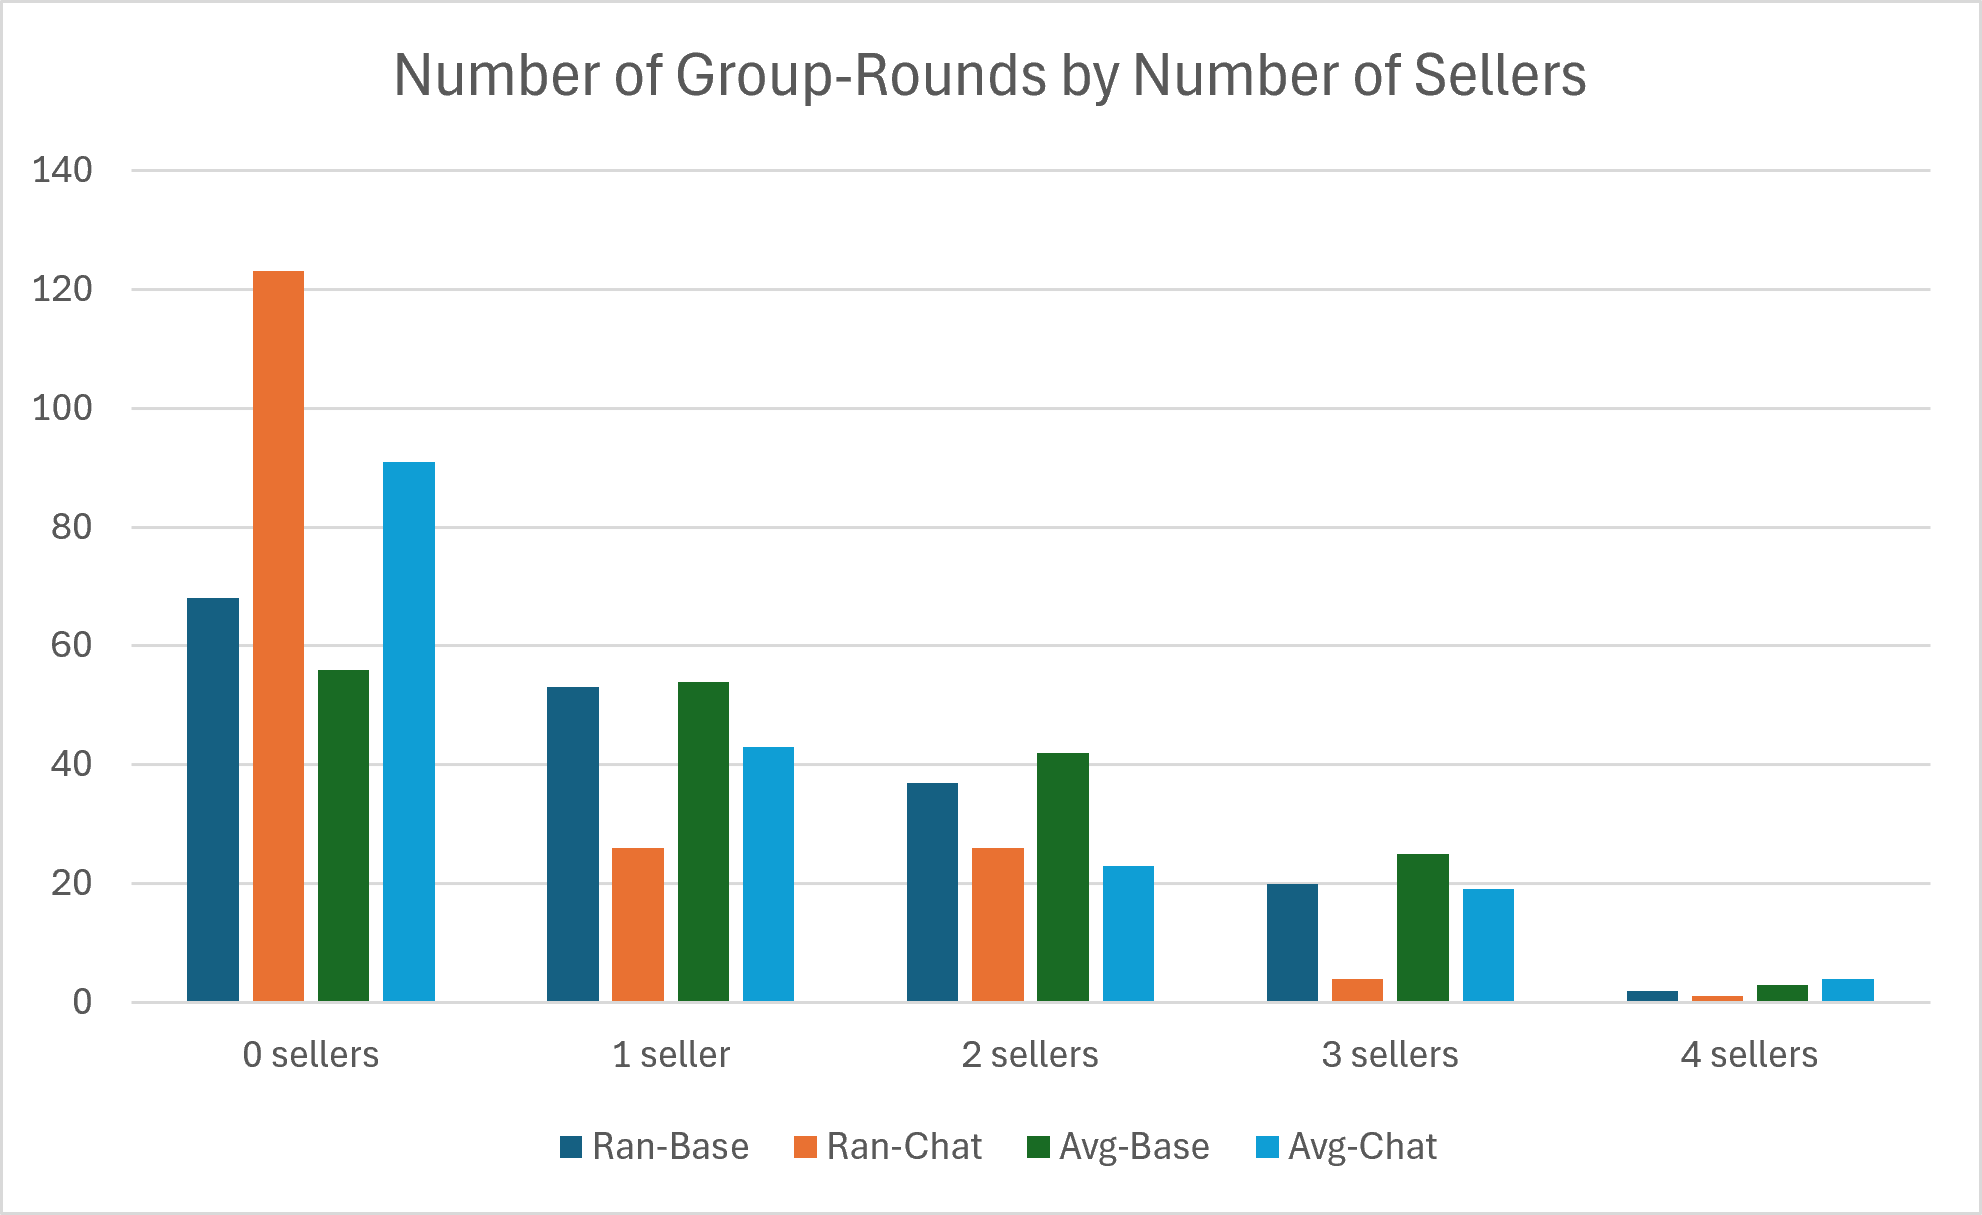
\includegraphics[width=9cm]{images/sellers_per_round.png}
\end{center}
\end{frame}



\begin{frame}{Selling Behavior}
\begin{center}
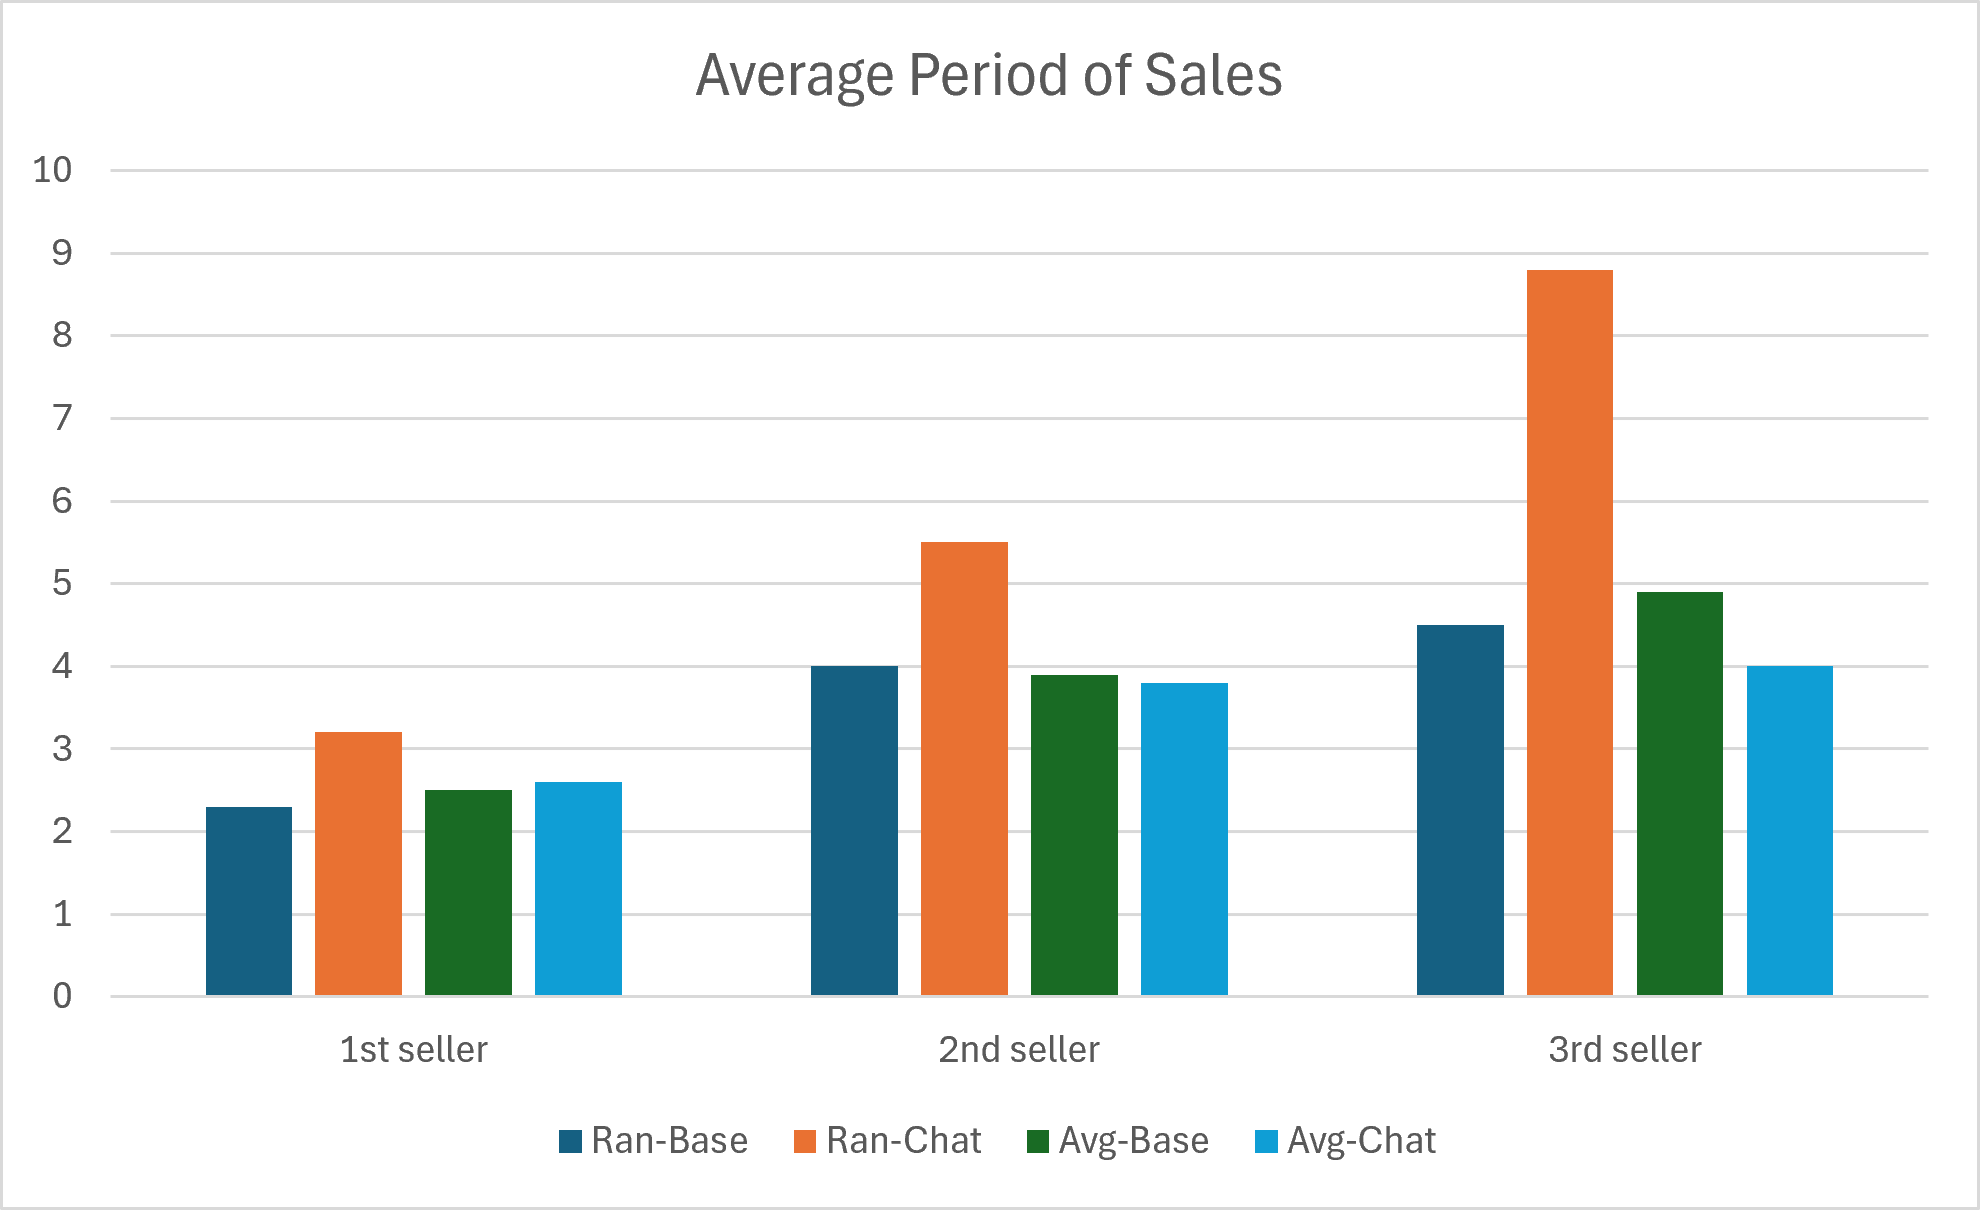
\includegraphics[width=9cm]{images/average_period_sales.png}
\end{center}
\end{frame}




\begin{frame}{1. Group-Round Level, Tobit Regression}

\begin{center}
\scalebox{0.5}{
\begin{tabular}{lcc}
   \tabularnewline \midrule \midrule
   Dependent Variable: & \multicolumn{2}{c}{Number of Sellers in Round}\\
   Model:               & (1)  & (2)\\
   \midrule
   \emph{Variables}\\
   Constant                  & 0.5603$^{**}$ & 0.8217$^{***}$\\
                             & (0.2664) & (0.2835)\\
   Bad state                 &  0.9827$^{***}$& 1.0138$^{***}$\\
                             &  (0.1551) & (0.1583)\\
   Round                     & -0.0738$^{**}$ & -0.0731$^{***}$\\
                             & (0.0256) & (0.0254)\\
   Treatment 2               & 0.4952$^{**}$ & -0.0529\\
                             & (0.2168) & (0.3193)\\
   Segment 2                 & -0.3539 & -0.6892$^{*}$\\
                             & (0.2486) & (0.3610)\\
   Segment 3                 & -1.0700$^{***}$ & -1.6068$^{***}$\\
                             & (0.3144) & (0.4742)\\
   Segment 4                 & -1.2829$^{***}$ & -1.7321$^{***}$\\
                             & (0.3027) & (0.3644)\\
   Treatment 2 $\times$ Segment 2     &   & 0.6672\\
                             &       & (0.4714)\\
   Treatment 2 $\times$ Segment 3     &   & 1.0339$^{*}$\\
                             &   & (0.6180)\\
   Treatment 2 $\times$ Segment 4     &  & 0.8684\\
                             &   & (0.5896)\\
   \midrule
   \emph{Fit statistics}\\
   Observations              & 720 & 720\\
   Log-likelihood            & -975.3 & -970.6\\
   \midrule \midrule
\end{tabular}   
}
\end{center}
\end{frame}


\begin{frame}{Tobit Takeaways}
\begin{itemize}
    \item \textbf{Chat segments} (3 \& 4) significantly decrease sellers by $\approx 1.1$--$1.3$
    \begin{itemize}
        \item Supports H1 --- communication reduces market runs
    \end{itemize}
    
    \item \textbf{Treatment 2} (average price liquidation) \textit{increases} sellers overall by $\approx 0.5$ per group-round (in Column 1) and $\approx 1.0$ per group-round when chat is allowed (in Column 2) 
    \begin{itemize}
        \item Supports H2 --- average price induces market runs
    \end{itemize}

    \item \textbf{Bad state} increases sellers by $\approx 1.0$ (participants understood signals)
    \item \textbf{Round} decreases sellers by $\approx 0.07$ (experience reduces runs)
\end{itemize}
\end{frame}

\begin{frame}{Tobit Takeaways}
\begin{center}
  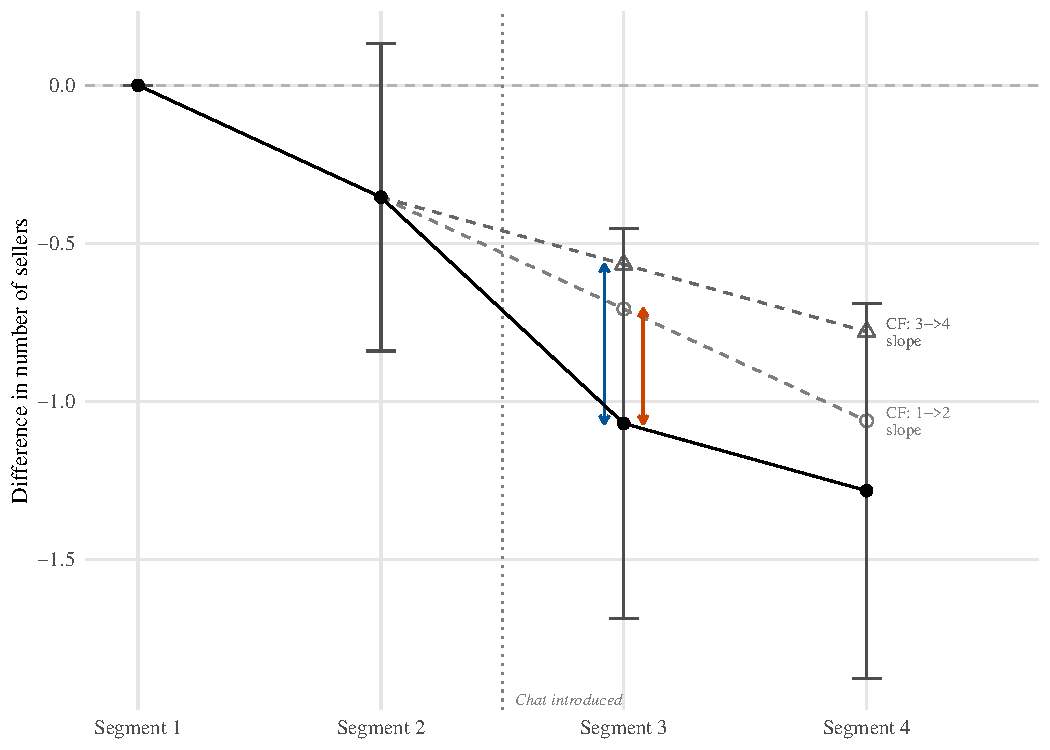
\includegraphics[width=0.7\linewidth]{did_segment_effects.pdf}
\end{center}
\end{frame}




\begin{frame}{2. Subject-Round Level, Rank-Ordered Logit (1) }

\begin{center}
\scalebox{0.5}{
\begin{tabular}{lcc}
   \tabularnewline \midrule \midrule
   Dependent Variable: & \multicolumn{2}{c}{Order of Sellers in Round}\\
   Model:               & (1)  & (2)\\
   & Sellers Only & All Participants \\
   \midrule
   Age                      & 0.0215 & 0.0211 \\
                            & (0.0567) & (0.0237) \\
   Female                   & -0.2371$^{**}$ & -0.0587 \\
                            & (0.0933) & (0.0525) \\
   Extraversion             & -0.0103 & -0.0106 \\
                            & (0.0597) & (0.0291) \\
   Agreeableness            & -0.1500$^{***}$ & -0.0302 \\
                            & (0.0556) & (0.0251) \\
   Conscientiousness        & 0.2973$^{***}$ & 0.0897$^{**}$ \\
                            & (0.0823) & (0.0449) \\
   Neuroticism              & -0.0282 & 0.0377$^{*}$ \\
                            & (0.0509) & (0.0228) \\
   Openness                 & 0.0372 & 0.0233 \\
                            & (0.0337) & (0.0161) \\
   Impulsivity              & 0.0491 & 0.0172 \\
                            & (0.0594) & (0.0315) \\
   State anxiety            & 0.1622$^{***}$ & 0.0515$^{***}$ \\
                            & (0.0440) & (0.0193) \\
   Risk tolerance           & 0.0444 & -0.0482$^{*}$ \\
                            & (0.0462) & (0.0258) \\
   \midrule
   \multicolumn{3}{l}{\emph{Coefficients are log-hazard ratios.}} \\
    \multicolumn{3}{l}{\emph{continued on next page}} \\
\end{tabular}   
}
\end{center}
\end{frame}

\begin{frame}{2. Subject-Round Level, Rank-Ordered Logit (2)}

\begin{center}
\scalebox{0.5}{
\begin{tabular}{lcc}
   \tabularnewline \midrule \midrule
   Dependent Variable: & \multicolumn{2}{c}{Order of Sellers in Round}\\
   Model:               & (1)  & (2)\\
   & Sellers Only & All Participants \\
   \midrule
   Fear                 & 0.0218 & 0.0064 \\
                            & (0.0871) & (0.0240) \\
   Anger                & 0.0001 & -0.0156$^{*}$ \\
                            & (0.2349) & (0.0094) \\
   Contempt             & 0.0340 & -0.0015 \\
                            & (0.0446) & (0.0125) \\
   Disgust              & 0.1491$^{**}$ & 0.0049 \\
                            & (0.0594) & (0.0068) \\
   Joy                  & -0.2149$^{**}$ & 0.0313 \\
                            & (0.0964) & (0.0202) \\
   Sadness              & 0.0087 & -0.0051 \\
                            & (0.0588) & (0.0097) \\
   Surprise             & 0.0791 & -0.0184 \\
                            & (0.0726) & (0.0260) \\
   Engagement           & 0.0871 & 0.0086 \\
                            & (0.0647) & (0.0174) \\
   Valence              & 0.1218 & -0.0486$^{**}$ \\
                            & (0.1084) & (0.0239) \\
   \midrule
   \emph{Fit statistics} & & \\
   Observations             & 486 & 2,845 \\
   Strata                   & 202 & 720 \\
   Concordance              & 0.688 & 0.670 \\
   Log-lik.                 & -221.3 & -2227.4 \\
   \midrule \midrule
   \multicolumn{3}{l}{\emph{Coefficients are log-hazard ratios.}} \\
\end{tabular}   
}
\end{center}
\end{frame}


\begin{frame}{RO-Logit Takeaways}
\begin{itemize}
    \item \textbf{Personality traits} 
    \begin{itemize}
        \item Sell earlier (ranked higher) --- conscientiousness, anxiety
        \item Sell later (ranked lower) --- agreeableness
    \end{itemize}
\vspace{0.2in}
    \item \textbf{Facial Emotions} 
    \begin{itemize}
        \item Sell earlier (ranked higher) --- disgust
        \item Sell later (ranked lower) --- joy, valence 
    \end{itemize}
\end{itemize}
\end{frame}



\begin{frame}{3. Subject-Period Level, Cox Survival Analysis (1)}

\begin{center}
\scalebox{0.5}{
\begin{tabular}{lcc}
   \tabularnewline \midrule \midrule
   Dependent Variable: & \multicolumn{2}{c}{Asset sold in Period}\\
   Model:               & (1)  & (2)\\
   & Periods with Sale & ~~~All Periods~~~ \\
   \midrule
   Age                        & 1.0577$^{*}$ & 1.0243 \\
                              & (0.0309) & (0.0364) \\
   Female                     & 1.0243 & 0.9602 \\
                              & (0.2057) & (0.2358) \\
   Extraversion               & 1.0931 & 0.9463 \\
                              & (0.0736) & (0.0736) \\
   Agreeableness             & 0.8960 & 0.8815 \\
                              & (0.0837) & (0.0981) \\
   Conscientiousness          & 1.3798$^{***}$ & 1.4279$^{***}$ \\
                              & (0.1550) & (0.1938) \\
   Neuroticism                & 0.9979 & 1.0638 \\
                             & (0.0795) & (0.0985) \\
   Openness                   & 0.9689 & 1.0716 \\
                              & (0.0779) & (0.1058) \\
   Impulsivity                & 1.1661 & 1.2020 \\
                              & (0.1585) & (0.1936) \\
   State anxiety              & 1.4355$^{**}$ & 1.5462$^{**}$ \\
                              & (0.2393) & (0.3126) \\
   Risk tolerance              & 1.0036 & 0.9639$^{**}$ \\
                               & (0.0145) & (0.0161) \\
   \midrule
   \multicolumn{3}{l}{\emph{Coefficients are hazard ratios.}} \\
    \multicolumn{3}{l}{\emph{continued on next page}} \\
\end{tabular}   
}
\end{center}
\end{frame}



\begin{frame}{3. Subject-Period Level, Cox Survival Analysis (2)}

\begin{center}
\scalebox{0.5}{
\begin{tabular}{lcc}
   \tabularnewline \midrule \midrule
   Dependent Variable: & \multicolumn{2}{c}{Asset sold in Period}\\
   Model:               & (1)  & (2)\\
   & Periods with Sale & ~~~All Periods~~~ \\
   \midrule
   Fear                       & 0.9917 & 0.9821 \\
                              & (0.0300) & (0.0265) \\
   Anger                      & 0.9833 & 0.9694 \\
                             & (0.0362) & (0.0340) \\
   Contempt                  & 0.9973 & 0.9862 \\
                               & (0.0080) & (0.0088) \\
   Disgust                   & 0.9926 & 0.9711 \\
                              & (0.0301) & (0.0273) \\
   Joy                        & 0.9955 & 1.0166$^{*}$ \\
                              & (0.0087) & (0.0086) \\
   Sadness                    & 1.0211 & 1.0001 \\
                              & (0.0146) & (0.0130) \\
   Surprise                   & 1.0073 & 1.0123 \\
                              & (0.0245) & (0.0195) \\
   Engagement                  & 0.9984 & 0.9980 \\
                              & (0.0029) & (0.0028) \\
   Valence                    & 1.0092 & 0.9870$^{*}$ \\
                              & (0.0074) & (0.0074) \\
   \midrule
   \multicolumn{3}{l}{\emph{Coefficients are hazard ratios.}} \\
    \multicolumn{3}{l}{\emph{continued on next page}} \\
\end{tabular}   
}
\end{center}
\end{frame}



\begin{frame}{3. Subject-Period Level, Cox Survival Analysis (3)}

\begin{center}
\scalebox{0.5}{
\begin{tabular}{lcc}
   \tabularnewline \midrule \midrule
   Dependent Variable: & \multicolumn{2}{c}{Asset sold in Period}\\
   Model:               & (1)  & (2)\\
   & Periods with Sale & ~~~All Periods~~~ \\
   \midrule
    1 prior sale              & 0.7918 & 0.8240 \\
                             & (0.1291) & (0.1273) \\
   2 prior sales              & 0.3682$^{***}$ & 0.2411$^{***}$ \\
                             & (0.1278) & (0.0775) \\
   3 prior sales              & 1.8089 & 0.0504$^{***}$ \\
                              & (2.2096) & (0.0511) \\
   1 prior $\times$ 1 prev.   & 1.1547 & 1.1740 \\
                              & (0.2111) & (0.2092) \\
   2 prior $\times$ 1 prev.   & 2.3809$^{**}$ & 2.7914$^{***}$ \\
                              & (0.9540) & (1.0795) \\
   2 prior $\times$ 2 prev.   & 3.2424$^{**}$ & 3.2047$^{***}$ \\
                              & (1.4834) & (1.3875) \\
   Good Signal                  & 0.0187$^{***}$ & 0.0035$^{***}$ \\
                                & (0.0061) & (0.0010) \\
   Round                       & 0.9503$^{***}$ & 0.9416$^{***}$ \\
                              & (0.0170) & (0.0158) \\
   Segment 2                  & 0.6615$^{***}$ & 0.8468 \\
                             & (0.0852) & (0.1016) \\
   Segment 3                  & 0.5928$^{***}$ & 0.3359$^{***}$ \\
                              & (0.0799) & (0.0437) \\
   Segment 4                   & 0.4254$^{***}$ & 0.3289$^{***}$ \\
                               & (0.0524) & (0.0382) \\
   Treatment 2                 & 0.9168 & 1.1397 \\
                              & (0.1634) & (0.2448) \\
   \midrule
   \multicolumn{3}{l}{\emph{Coefficients are hazard ratios.}} \\
    \multicolumn{3}{l}{\emph{continued on next page}} \\
\end{tabular}   
}
\end{center}
\end{frame}



\begin{frame}{3. Subject-Period Level, Cox Survival Analysis (4)}

\begin{center}
\scalebox{0.5}{
\begin{tabular}{lcc}
   \tabularnewline \midrule \midrule
   Dependent Variable: & \multicolumn{2}{c}{Asset sold in Period}\\
   Model:               & (1)  & (2)\\
   & Periods with Sale & ~~~All Periods~~~ \\
   \midrule
   \emph{Fit statistics}   & & \\
   Observations               & 2,013 & 13,590 \\
   Events                     & 659 & 659 \\
   Participants               & 87 & 95 \\
   Log-likelihood             & -3449.8 & -4393.0 \\
   \midrule
\end{tabular}   
}
\end{center}
\end{frame}



\begin{frame}{Cox Survival Takeaways}
\begin{itemize}
    \item \textbf{Personality traits} 
    \begin{itemize}
        \item More likely to sell   --- conscientiousness, anxiety
        \item Less likely to sell  --- risk tolerance
    \end{itemize}
\vspace{0.2in}
    \item \textbf{Facial Emotions} --- not significant

\vspace{0.2in}
    \item \textbf{Cascade, Experience, and Information} 
        \begin{itemize}
        \item More likely to sell   --- immediate prior sales
        \item Less likely to sell  --- good signal, later rounds, chat segments
    \end{itemize}
\end{itemize}
\end{frame}




\begin{frame}{4. First and Rushed Sellers, Cox Survival Analysis (1)}

\begin{center}
\scalebox{0.5}{
\begin{tabular}{lcc}
   \tabularnewline \midrule \midrule
   Dependent Variable: & \multicolumn{2}{c}{Asset sold in Period}\\
   Model:               & (1)  & (2)\\
   & Periods with 1st Sale & Periods after 1st Sale \\
   \midrule
   Age                        & 1.0577$^{*}$ & 1.0243 \\
                              & (0.0309) & (0.0364) \\
   Female                     & 1.0243 & 0.9602 \\
                              & (0.2057) & (0.2358) \\
   Extraversion               & 1.0931 & 0.9463 \\
                              & (0.0736) & (0.0736) \\
   Agreeableness             & 0.8960 & 0.8815 \\
                              & (0.0837) & (0.0981) \\
   Conscientiousness          & 1.3798$^{***}$ & 1.4279$^{***}$ \\
                              & (0.1550) & (0.1938) \\
   Neuroticism                & 0.9979 & 1.0638 \\
                             & (0.0795) & (0.0985) \\
   Openness                   & 0.9689 & 1.0716 \\
                              & (0.0779) & (0.1058) \\
   Impulsivity                & 1.1661 & 1.2020 \\
                              & (0.1585) & (0.1936) \\
   State anxiety              & 1.4355$^{**}$ & 1.5462$^{**}$ \\
                              & (0.2393) & (0.3126) \\
   Risk tolerance              & 1.0036 & 0.9639$^{**}$ \\
                               & (0.0145) & (0.0161) \\
   \midrule
   \multicolumn{3}{l}{\emph{Coefficients are hazard ratios.}} \\
    \multicolumn{3}{l}{\emph{continued on next page}} \\
\end{tabular}   
}
\end{center}
\end{frame}


\begin{frame}{4. First and Rushed Sellers, Cox Survival Analysis (2)}

\begin{center}
\scalebox{0.5}{
\begin{tabular}{lcc}
   \tabularnewline \midrule \midrule
   Dependent Variable: & \multicolumn{2}{c}{Asset sold in Period}\\
   Model:               & (1)  & (2)\\
   & Periods with 1st Sale & Periods after 1st Sale \\
   \midrule
   Fear                      & 1.0193 & 2.2148$^{***}$   \\
                             & (0.0331) & (0.6529)  \\
   Anger                     & 0.9751 & 0.7359  \\
                             & (0.0423) & (0.1383)   \\
   Contempt                  & 1.0079 & 1.0096  \\
                             & (0.0090) & (0.0152)   \\
   Disgust                   & 1.0132 & 1.1025  \\
                             & (0.0337) & (0.0684)  \\
   Joy                       & 1.0007 & 1.0518$^{*}$  \\
                             & (0.0105) & (0.0289)   \\
   Sadness                   & 1.0025 & 0.9824   \\
                             & (0.0204) & (0.0261)   \\
   Surprise                  & 1.0004 & 0.3576$^{***}$  \\
                             & (0.0249) & (0.1262)   \\
   Engagement                & 0.9952 & 0.9976   \\
                             & (0.0035) & (0.0086)   \\
   Valence                   & 1.0032 & 0.9728   \\
                             & (0.0090) & (0.0228)   \\
   \midrule
   \multicolumn{3}{l}{\emph{Coefficients are hazard ratios.}} \\
    \multicolumn{3}{l}{\emph{continued on next page}} \\
\end{tabular}   
}
\end{center}
\end{frame}




\begin{frame}{4. First and Rushed Sellers, Cox Survival Analysis (3)}

\begin{center}
\scalebox{0.5}{
\begin{tabular}{lcc}
   \tabularnewline \midrule \midrule
   Dependent Variable: & \multicolumn{2}{c}{Asset sold in Period}\\
   Model:               & (1)  & (2)\\
   & Periods with 1st Sale & Periods after 1st Sale \\
   \midrule
    Good Signal               & 0.0025$^{***}$ & 0.0160$^{***}$   \\
                             & (0.0012) & (0.0171)  \\
   Round                     & 0.9463$^{**}$ & 0.9042$^{*}$ \\
                             & (0.0215) & (0.0506)   \\
   Segment 2                 & 0.5906$^{***}$ & 0.5676  \\
                             & (0.0936) & (0.2582)   \\
   Segment 3                 & 0.3889$^{***}$ & 0.5204$^{*}$  \\
                             & (0.0642) & (0.1778)   \\
   Segment 4                 & 0.4022$^{***}$ & 0.5775$^{*}$ \\
                             & (0.0634) & (0.1898)   \\
   Treatment 2               & 0.8548 & 1.4259  \\
                             & (0.1915) & (0.4409)  \\
   \midrule

      \emph{Fit statistics} & &  \\
   Observations              & 1,183 & 1,082   \\
   Events                    & 467 & 101  \\
   Participants              & 83 & 88   \\
   Log-likelihood            & -2220.9 & -492.3  \\
      \midrule
         \multicolumn{3}{l}{\emph{Coefficients are hazard ratios.}} \\
   \\
\end{tabular}   
}
\end{center}
\end{frame}

\begin{frame}{Additional Cox Survival Takeaways}
\begin{itemize}
    \item \textbf{Personality traits} 
    \begin{itemize}
        \item More likely to sell first  --- conscientiousness, anxiety
        \item More likely to follow   --- conscientiousness, anxiety
        \item Less likely to follow    --- risk tolerance
    \end{itemize}
\vspace{0.2in}
    \item \textbf{Facial Emotions}
    \begin{itemize}
        \item More likely to sell first  --- not significant
        \item More likely to follow   --- fear
        \item Less likely to follow   --- surprise
    \end{itemize}
\vspace{0.2in}
    \item \textbf{Cascade, Experience, and Information} 
        \begin{itemize}
        \item Less likely to sell first  --- good signal, later rounds, chat segments
        \item Less likely to follow  --- good signal only! No significant effects by experience or chat
    \end{itemize}
\end{itemize}
\end{frame}




\begin{frame}{5. First Sales, Pooled OLS}

\begin{center}
\scalebox{0.5}{
\begin{tabular}{lcc}
   \tabularnewline \midrule \midrule
   Dependent Variables: 
    & {Belief at First Sale} & {Period of First Sale} \\ 
   Model:         & (1)             & (2)     \\  
   \midrule
   \emph{Variables}\\
   Constant       & 0.4862$^{***}$   & 1.972$^{***}$\\   
                        & (0.0269)           & (0.2891)\\   
    Bad State      & -0.1034$^{***}$ & 0.5257$^{***}$\\   
                 & (0.0159)        & (0.1502)\\   
   Round       & -0.0054          & 0.0263\\   
              & (0.0033)         & (0.0337)\\  
  Treatment 2    & 0.0278        & -0.2058\\   
                & (0.0223)        & (0.2520)\\   
   Segment 2   & -0.0157         & 0.2938\\   
                   & (0.0290)       & (0.3200)\\   
   Segment 3   & -0.0715$^{**}$   & 0.3530\\   
                 & (0.0326)      & (0.2798)\\   
   Segment 4  & -0.0711$^{**}$        & 0.4880\\   
                  & (0.0313)      & (0.4144)\\    
   \midrule
   \emph{Fit statistics}\\
   Observations    & 382           & 382\\  
   R$^2$           & 0.17561        & 0.04696\\  
   \midrule \midrule
\end{tabular}
}
\end{center}
\end{frame}



\begin{frame}{First-Sale OLS Takeaways}
\begin{itemize}
    \item \textbf{Belief at First Sale} 
    \begin{itemize}
        \item Less than 0.5
        \item Lower in Bad state and under chat
        \item No significant effect by experience
    \end{itemize}
\vspace{0.2in}
    \item \textbf{Period of First Sale}
    \begin{itemize}
        \item Approx. 2
        \item Higher in Bad state
        \item No significant effects by experience or chat
    \end{itemize}
\end{itemize}
\end{frame}


\begin{frame}{6. Welfare, Pooled OLS (1)}

\begin{center}
\scalebox{0.5}{
\begin{tabular}{lc}
   \tabularnewline \midrule \midrule
   Dependent Variables: 
    & Welfare \\ 

   \midrule
   \emph{Variables}\\
   Constant            & 0.9482$^{***}$\\   
                       & (0.0832)\\   
   Round               & 0.0090$^{***}$\\   
                       & (0.0033)\\   
   Segment   2       & 0.0772$^{**}$\\   
                       & (0.0304)\\   
   Segment   3       & 0.1077$^{***}$\\   
                       & (0.0343)\\   
   Segment   4       & 0.1307$^{***}$\\   
                       & (0.0251)\\   
   Age                 & -0.0046$^{**}$\\   
                       & (0.0022)\\   
   Female      & -0.0128\\   
                       & (0.0130)\\   
   Treatment 2        & -0.0193\\   
   \midrule \midrule
       \multicolumn{2}{l}{\emph{continued on next page}} \\
\end{tabular}
}
\end{center}
\end{frame}

\begin{frame}{6. Welfare, Pooled OLS (2)}

\begin{center}
\scalebox{0.5}{
\begin{tabular}{lc}
   \tabularnewline \midrule \midrule
   Dependent Variables: 
    & Welfare \\ 

   \midrule
   \emph{Variables}\\
   Extraversion        & 0.0062$^{**}$\\   
                       & (0.0030)\\   
   Agreeableness       & 0.0056\\   
                       & (0.0056)\\   
   Conscientiousness   & -0.0103$^{**}$\\   
                       & (0.0051)\\   
   Neuroticism         & -0.0016\\   
                       & (0.0042)\\   
   Openness            & 0.0044\\   
                       & (0.0041)\\   
   Impulsivity         & -0.0102\\   
                       & (0.0086)\\   
    State anxiety      & -0.0198$^{**}$\\   
                       & (0.0098)\\   

   Risk tolerance     & -0.0004\\   
                       & (0.0006)\\   
   \midrule
   \emph{Fit statistics}\\
   Observations        & 1,440\\  
   R$^2$               & 0.14616\\  
   \midrule \midrule
\end{tabular}
}
\end{center}
\end{frame}

\begin{frame}{Welfare OLS Takeaways}
\begin{itemize}
    \item \textbf{Positive Effects} 
    \begin{itemize}
        \item Chat
        \item Experience
        \item Extraversion
    \end{itemize}
\vspace{0.2in}
    \item \textbf{Negative Effects}
    \begin{itemize}
        \item Age
        \item Conscientiousness
        \item Anxiety
    \end{itemize}
\end{itemize}
\end{frame}

\begin{frame}{7. Luck in Treatment 1 (Random Price)}
Does being ``unlucky'' in a liquidation event predict future selling?


\begin{columns}[T]
\begin{column}{0.55\textwidth}
\begin{itemize}
    \item Reference: Payoff = 2 (unluckiest)
    \item Group-round fixed effects
    \item Treatment 1 only
    \item Prior sales: number of sales made by the participant in the past
\end{itemize}
\end{column}
\begin{column}{0.4\textwidth}

\centering
\scriptsize
\begin{tabular}{@{}lc@{}}
   \midrule \midrule
   Dep.\ Var:    & Sold next round \\
   \midrule
   Payoff 4                & $-$0.035\\
                           & (0.032)\\
   Payoff 6                & $-$0.066\\
                           & (0.044)\\
   Payoff 8                & $-$0.092$^{*}$\\
                           & (0.053)\\
   Prior sales             & 0.015$^{**}$\\
                           & (0.007)\\
   \midrule
   Group-Round FE          & Yes\\
   Observations            & 416\\
   R$^2$                   & 0.420\\
   \midrule \midrule
   \multicolumn{2}{l}{\tiny\emph{***: 0.01, **: 0.05, *: 0.1}}\\
\end{tabular}
\end{column}
\end{columns}
\end{frame}

\begin{frame}{Luck Plot}
    \begin{figure}
        \centering
        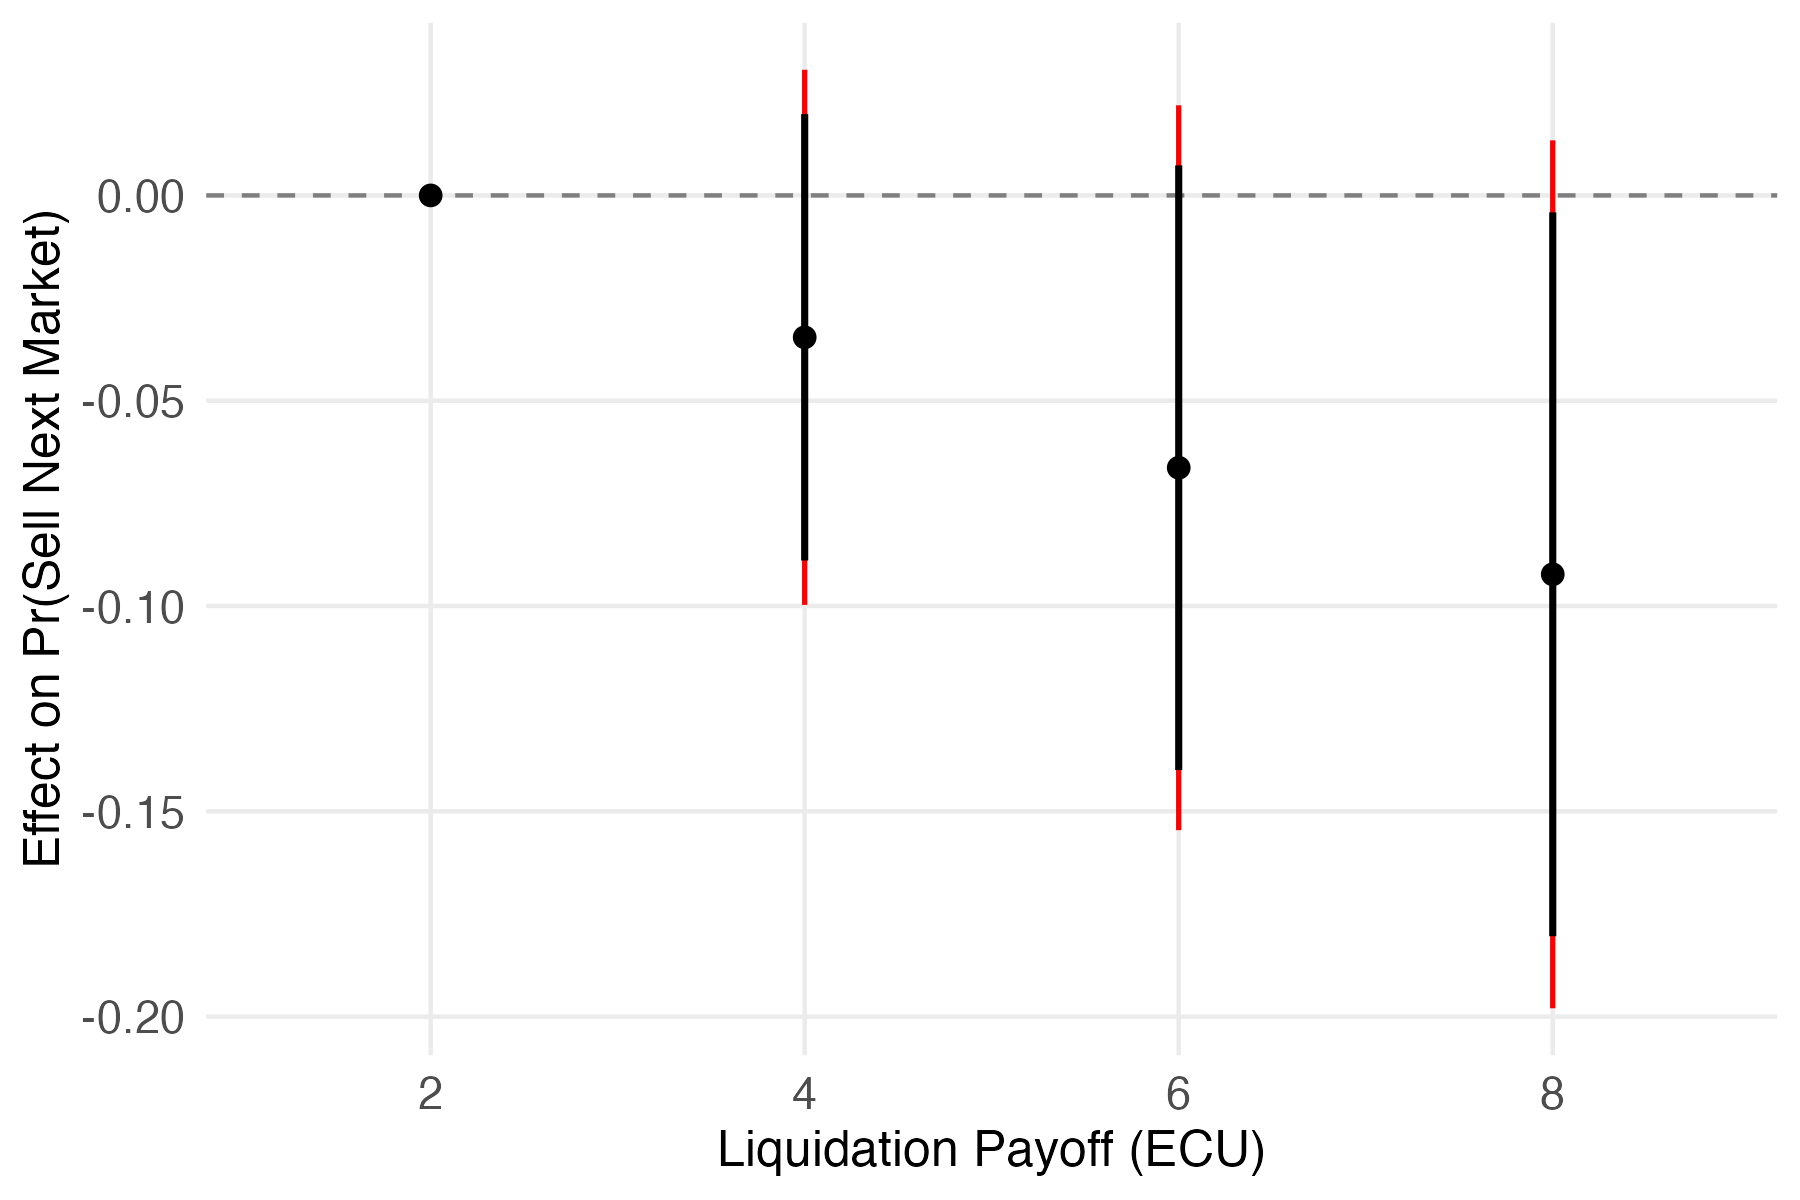
\includegraphics[width=0.8\linewidth]{holdout_payoff_coefficients.png}
        \label{fig:luck}
    \end{figure}
\end{frame}



\begin{frame}{Luck Takeaways}
\begin{itemize}
    \item Receiving payoff of 8 (vs.\ 2) $\rightarrow$ \textbf{9.2\% less likely} to sell next round
    \item Coefficients are \textbf{monotonically decreasing}: luckier $\rightarrow$ less likely to sell
    \item Payoffs of 4 and 6 (vs.\ 2) not significant
    \item Being unlucky causes more future selling, even though round states and signals are independent
    \item Evidence against purely rational updating
\end{itemize}
\end{frame}


%%%%%%%%%%%%%%%%%%%%%%%%%%%%%%%%%%%%%
% CONCLUSION
%%%%%%%%%%%%%%%%%%%%%%%%%%%%%%%%%%%%%

\begin{frame}{Summary of Hypothesis Tests}
\begin{center}
\begin{tabular}{lcc}
\toprule
\textbf{Hypothesis} & \textbf{Predicted Effects} & \textbf{Evidence} \\
\midrule
H1: Chat treatment & negative & \textcolor{green!50!black}{Supported} \\
H2: Average treatment & positive & \textcolor{green!50!black}{Supported} \\
H3: Anxiety, conscientiousness  & positive & \textcolor{green!50!black}{Supported} \\
H3: Risk tolerance & negative & \textcolor{green!50!black}{Supported} \\
H3: Impulsivity & positive & \textcolor{red}{Not supported}\\
H3: Openness, agreeableness & negative & \textcolor{red}{Not supported}\\
H4: Joy, valence & negative & \textcolor{orange}{Mixed} \\
H4: Fear, disgust  & positive & \textcolor{orange}{Mixed}\\
H4: Anger, engagement & positive & \textcolor{red}{Not supported}\\
\bottomrule
\end{tabular}
\end{center}
\end{frame}


\begin{frame}{Conclusion}
\begin{itemize}
    \item Individual psychological factors are significant predictors of market run participation
    \item \textbf{Traits:} Conscientiousness and anxiety increase selling; risk tolerance decreases it
    \item \textbf{Emotions:} Joy, valence (negative) Fear, disgust (positive)    \item \textbf{Cascades:} Recent sales trigger panic despite providing no new information
    \item \textbf{Communication:} Chat reduces market runs significantly
\end{itemize}

\vspace{0.3cm}
\textbf{Next Steps:}
\begin{itemize}
    \item Text analysis
\end{itemize}
\end{frame}


\begin{frame}{Policy implications}
\begin{itemize}
    \item Communication increases market stability
    \item Language that avoids stimulating negative emotions may prevent runs
    \item Batch trading with average price induces runs
    \item Prices are not solely driven by fundamentals
\end{itemize}
\end{frame}


\begin{frame}{Future Work}
\begin{itemize}
    \item Real-time pricing
    \item Other measures of emotions
    \item Survey professional traders on personality traits
    \begin{itemize}
        \item Use sufficient statistics to compare with experimental panic sellers
    \end{itemize}
    \item Test interventions to mitigate negative emotional reactions
    \item Semi-private signals for a more realistic market setting
    \begin{itemize}
        \item Sales would then provide additional information beyond price changes
    \end{itemize}
\end{itemize}

\vspace{1cm}
\centering
\Large Thank you!
\end{frame}


\begin{frame}[allowframebreaks]{References}
\bibliographystyle{aea}
\scriptsize
\bibliography{refs}
\end{frame}

\end{document}
